\begin{tframe}{CNN - Architecture}

The net is based on LeNet and consists of eight layers, as shown in the following image.

\begin{figure}[h]
	\begin{center}
		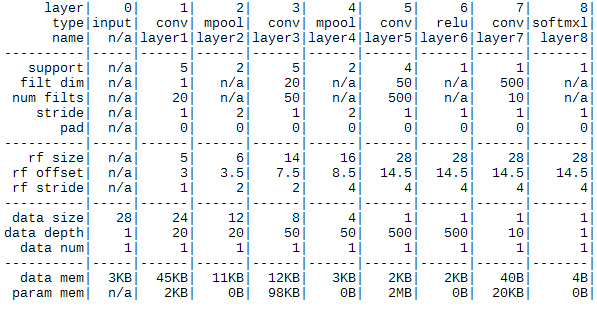
\includegraphics[width=1\textwidth]{img/cnn.png}
	\end{center}
	\label{fig:cnn}
\end{figure}

\end{tframe}

\begin{tframe}{CNN - Settings}

\vspace{0.1in}
\vspace{0.1in}
\vspace{0.1in}

\begin{itemize}
\item Number of epochs 30
\item Learning rate initialized to 0.001
\item Batch size of 100
\item Softmax log-loss as a cost function
\item SGD with momentum initialized to 0.9
\item Weight decay of 0.0005
\end{itemize}


\end{tframe}